\chapter{Timeline}
\label{chap:plan}
% Work Plan

This final chapter of this report describes the timeline, considering both the work that has been done up to the current date and the plan for the next two years of research.
While the previous chapter described the methodology and evaluation that is planned, here we describe when each part of the project is expected to be addressed.

\section{Work to date}
% until now: what has been done
% - initial experiments
% - formalisation and problem definition
% - data

During the first year, several activities have been done.
Some have been done as initial explorations in the field of research, understanding what other researchers have done, ``getting the hands dirty'' with data and NLP tools.
And their function within the PhD project has been to lead to the Research Questions that we described earlier.
Some other activities have been done to kick start the future experimentation, for example doing data collection of news articles or by beginning to implement some of the stages of the processing pipeline that will be used.
% , with the goal to find and formulate proper Research Questions and to prepare the execution of the proposal.


\subsection{Paper reproduction~\cite{bountouridis2018explaining}}
% Experiment 1
% what
We started by analysing the paper from~\citet{bountouridis2018explaining} which presents a methodology to analyse how much information overlaps between different similar documents, identifying points of information that are corroborated or omitted.
% why
We wanted to analyse this resource because it seems to be going in the broad direction of our project, analysing different presentations in the news of the same event.

% how
The paper has been analysed and reproduced, to get a deep understanding of how it works. The implementation started with the code publicly provided by the authors,\footnote{\url{https://github.com/dbountouridis/InCredible}} but its incompleteness in some stages of the processing (e.g., the creation of the article-level cliques, and all the specific hyperparameters of the algorithms used) required integrating the codebase.\footnote{\url{https://github.com/MartinoMensio/InCredible}}

% limitations
With the experiments reproduced, we have been able to inspect the cliques of documents and sentences identified by the model, seeing the following limitations:

\begin{itemize}
    % \item Their demo\footnote{\url{http://fairnews.ewi.tudelft.nl/InCredible/}} just shows one specific article as main and one specific clique (not very interesting)
    \item The \emph{document clustering} sometimes splits similar articles over different clusters, or in some cases has different stories that talk about a different detail within the same cluster (e.g., when a news story re-emerges because further details are discovered).
    This can be a consequence of having TF-IDF as the underlying method to represent the documents.
    This method is fast and efficient for coarse topic detection, because it is based on bag-of-words which works well with specific terms that distinguish the topics.
    But when we need to have a finer-grained clustering such in this case, the limitation of such method may surface because the terms of two political events with the same entities mentioned result in having similar feature vectors.
    \item The \emph{sentence clustering} method provided just says that two sentences are similar, but does not point to which specific words are responsible for the similarities and differences. This would require a framing analysis that in this paper is not included. Furthermore, sentences in a clique are very similar and no big differences have been observed because the similarity metrics is based again on TF-IDF. This method is not robust enough to the usage of synonyms and other variations on the linguistic surface, while at the same time is unable to distinguish two sentences that use the same words but have different meanings because of the sentence structure, so it makes selecting a threshold value very difficult.
    \item The \emph{clique algorithms} are not the best choice for doing clustering when we have the information of how much similar two items are (a real-value is available from the similarity metric). The approach considers an unweighted version of the similarity graph by using a threshold (weights are just used to select the most appropriate clique during their creation), but instead dealing with the original weighted graph would allow better clustering techniques. %, like agglomerative clustering
\end{itemize}


% In addition to these problems, the model described is based on TF-IDF which is not as robust with changes on the linguistic surface (as we saw in the next experiment).
% Models flourished
% This is the motivation for 5.1.2

% And also, it uses the similarity between TF-IDF just with a threshold, modelling the graph and cliques as unweighted (the weights are just used to select the most appropriate clique during their creation).

% role of this experiment
This experiment helped to see the limitation of this type of work, that belongs to the \emph{similarity} area of research (Section~\ref{sec:lit_relationships}).
This paper provides a great way to analyse the overlap between articles and extracts pieces that have been omitted or that are corroborated, but does not investigate further in the reason behind the selection of what to include or not.
This opened up for further work to:
\begin{enumerate}
    \item investigate how to better represent the documents to provide meaningful similarity metrics;
    \item investigate the works that analyse framing theories and detection;
    \item experiment with document and sentence clustering to bring up differences;
    \item collect data from more recent articles that would be more relevant and interesting.
\end{enumerate}
% \emph{i)} , \emph{ii)} , \emph{iii)} , and \emph{iv)} g.

Apart from these limitations, we are building our processing pipeline on top of this type of analysis, that links together news articles at different granularity levels (documents, sentences, words).
This gives us the opportunity to use features from multiple articles for the next stage of automated detection of framing techniques.


\subsection{Models for similarity analysis}
% Experiment 2
% what
Moving to the problem of representing documents and sentences in a way that captures more the semantic similarity, we decided to analyse closer the existing works, including word embeddings and language models.
We wanted to see in practice how the usage of different representation models would affect the measurements of similarity, experimenting with a small set of articles. 
% finding and exploring more advanced methods to find the similarity between texts by using language models, we experimented on how to use these methods.
% why?
Having a solid base for computing the distances between articles and sentences is a pillar for comparing different articles. The applications of similarity range from document clustering to identification of omitted pieces of information in a cluster, therefore it is very important to use a proper method that is not fooled by the usage of synonyms and other linguistic variations in communicating the same information. To study the differences in the language of framing we first need to be able to tell whether two pieces of text are discussing the same information, and distinguish properly degrees of similarity.

% how?
% Specifically on the sentence level, we experimented to see how different models were able to pick similar sentences, by setting up a small benchmark.
We set up a small benchmark where the goal is to find the most similar pairs of sentences coming from selected pairs of news articles which cover the same event. Each model candidate has to tell which 10 most similar pairs of sentences has found, one from one article and one from the other.
The pairs of articles have been chosen manually, by considering three constraints: \textit{i)} description of the same event, \textit{ii)} from different news outlets, \textit{iii)} published near in time, with a maximum distance of one day.
Each model would extract the most similar 10 pairs, and we then compare the pairs provided and their relative order.

The selected models used in the benchmark are the following:
\begin{itemize}
    \item \textbf{TF-IDF}: with a feature size of 2000, with a preprocessing made of lowercasing and tokenizing, without lemmatisation;
    \item \textbf{GloVe-average}: considering GloVe word embeddings trained on the CommonCrawl dataset, and doing an average of the vectors over the sentence;\footnote{\url{https://spacy.io/models/en\#en_core_web_lg}}
    \item \textbf{BERT}: using the most popular embeddings provided by Google Research~\cite{devlin2018bert} with the base uncased pre-trained weights;\footnote{\url{https://spacy.io/models/en-starters\#en_trf_bertbaseuncased_lg}}
    \item \textbf{USE}: using sentence embeddings coming from Universal Sentence Encoder~\cite{cer2018universal} which has been specifically trained for sentence similarity\footnote{\url{https://tfhub.dev/google/universal-sentence-encoder/}}
\end{itemize}

In all the cases, the representations from these models have been compared with the cosine similarity.
For each pair of sentences that was provided by any of the models, we listed by manual analysis which differences were contained, in terms of details that changed, or different words used.


\begin{figure}[!htb]
    \centering
    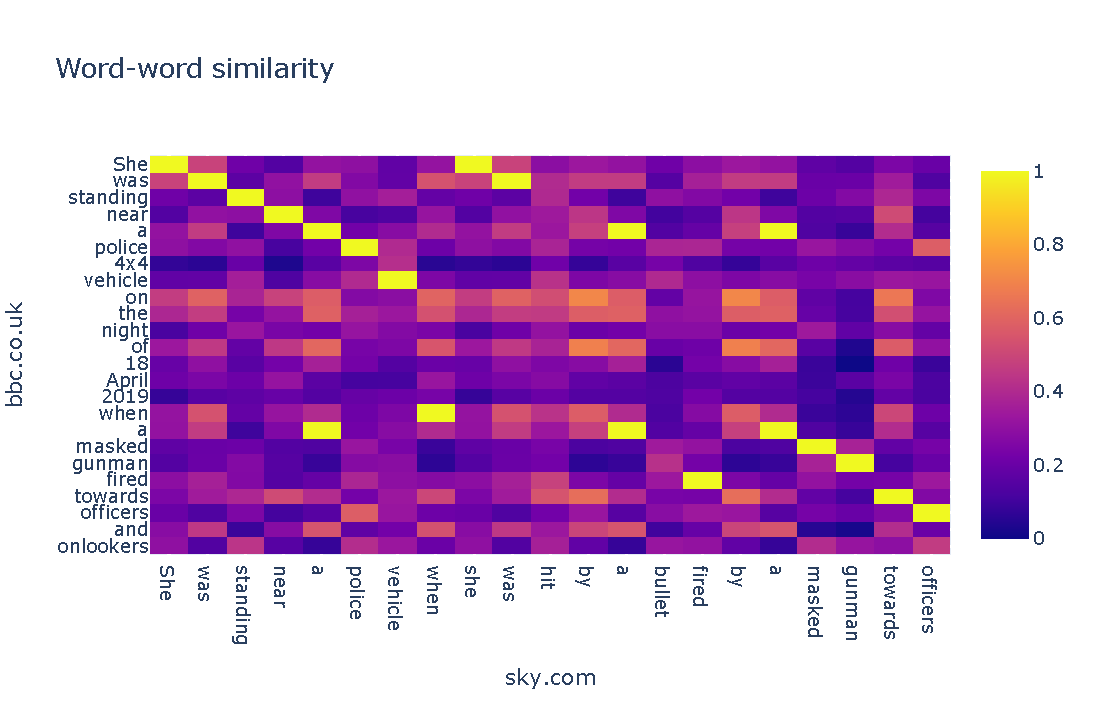
\includegraphics[width=0.9\linewidth]{figures/lyra.pdf}
    \caption{The comparison between two sentences, one from the BBC and the other from Sky News, where multiple differences exist.}
    \label{fig:lyra}
\end{figure}

An example can be seen in Figure~\ref{fig:lyra} that shows a sentence from the BBC\footnote{\url{https://www.bbc.co.uk/news/uk-england-hereford-worcester-51791346}} and one from Sky News,\footnote{\url{https://www.dailymail.co.uk/news/article-8088805/Britons-facing-heavy-downpours-four-inches-rain-50mph-winds-set-batter-UK.html}} where the differences are the following:

\begin{itemize}
    \item the detail ``4x4'' just appears on the BBC article;
    \item the detail ``on the night of 18 April 2019'' just appears on the BBC article;
    \item Active vs passive sentence ``a masked gunman fired'' vs ``she was hit by a bullet fired by a masked gunman'';
    \item the detail ``a bullet'' just appears in the Sky article;
    \item ``Towards officers and onlookers'' vs ``towards officers'': in the second, the targets of the gunman are just the officers.
\end{itemize}

With this kind of information on the number, type and magnitude of changes contained in different pairs of sentences, we can get a qualitative idea of how the measures of similarity coming from the different models are representative of the effective differences. If a model scores more similar a pair of sentences that appear to us to be less related than another pair, that is a negative sign for that model. 


% Observations
% \todo{rewrite better the observations}
The observations that we have for the TF-IDF model is that the feature size changes the results a lot.
It requires to be computed on a set of documents all together (which also changes which features are selected), and it is not possible to encode an additional document without changing the representation of the already encoded documents.
We also see that the type of pre-processing affects the results: without a lemmatization step to the pipeline, it is sufficient to change the verb tense to have a different term.
Given these limitations, we find that sentences that are very similar in the meaning but have some differences in the linguistic surface see a drop in their similarity with this model.

Instead considering GloVe-average, we observe in some cases that the measure of similarity provided does not capture substantial changes in the meaning. The problem is that, while it can use wordwise similarity quite well, the sentence structure is not accounted for its representation. The representation is a simple average of the word vectors (e.g. ``Luke insulted John'' results in being equal to ``John insulted Luke'').

For the language models (BERT and USE models), we see a big improvement in the pairs of sentences that come as more similar.
% The values provided are very similar. This per-se is not a problem if some geometric properties are valid (ordering, proportions)
We observe that USE provides values less skewed to the higher end, distributing the similarity values more evenly. The numbers make more sense without any re-scaling technique, and therefore the heatmaps shown in this document come from this model.
It is also the only model considered that is purposely trained on a semantic similarity task, while the other models can provide similarity measures just because of how they represent language.


% \todo{an example of two pairs where we can see some of the limitations?}

% role of this experiment
This experiment shows the need for a similarity model that accounts for the semantics more than the linguistic surface. And given the continuous progress of language models, we need to be able to switch our choice relatively easily.
For example, by looking at the Semantic Textual Similarity benchmark,\footnote{\url{http://nlpprogress.com/english/semantic_textual_similarity.html}} at the moment the best model available is XLNet~\cite{yang2019xlnet} so we will use it for our future experiments.
% this means for us:
% - we need to use a similarity resistant to changes in the linguistic surface
% - we need a measure that is able to represent well the different levels of similarity
% - we must be able to switch the model used easily, in case new public benchmarks for STS show a different winner (example XLNet~\cite{yang2019xlnet}).

The purpose of this experiment is to have a good observation of how different types of models can be effective or not, and to experiment with them to drive the implementation of the processing pipeline.
% Benchmark, availability of code and maybe further measures on our system will decide the final ``winner''.
% Purpose: implementation and building of the pipeline.


\subsection{Sentence clustering and extraction of differences}
% Experiment 3
% what
The next experimentation that we have done regards the usage of the similarity values to group together sentences describing the same details and at the same time study the uniqueness of the words used.
% why
We have seen with the reproduction of the model from \citet{bountouridis2018explaining} that one big limitation of using cliquing techniques over unweighted graphs is that they do not exploit the full power of the distances available, which resulted in having fragmented clusters due to a choice of the ``similar-enough threshold'' that is disputable.
% We have also experimented with different embedding models and we want to use them
% \todo{from here on}
% This comes from the limitation of the first experiment of reproduction of the paper. (from experiment 1)
% (from experiment on similarity)

% how
With this idea, we retrieved some groups of articles that relate to the same event from Google Headlines, which aggregates and clusters together news articles from multiple sources.\footnote{\url{https://www.blog.google/products/news/new-google-news-ai-meets-human-intelligence/}}
These documents are processed with the SpaCy NLP Python library\footnote{\url{https://spacy.io/}} to split the documents into sentences and have available different NLP functions (e.g., tokenisation, POS tagging).

% 1. distance computation
Each of the sentences is then passed through a language model which creates a sentence embedding, in this case using the Universal Sentence Encoder because it showed to distribute the similarity values more evenly and is specifically trained for sentence similarity.

% 2. hierarchical clustering (example with diagram)
We then use agglomerative hierarchical clustering for different reasons:
\begin{itemize}
    \item it does not require the specification of the number of clusters wanted, we want to be flexible;
    \item we can truncate the clustering when we reach a certain level of distance between the clusters, or a certain number of clusters;
    \item We can see the evolution of many different features (e.g., number of clusters, size, internal cohesion) while performing the clustering step by step;
    \item we have a graphical representation (dendrogram) which helps to inspect and understand what is happening;
    \item it has widely been used for similar tasks (e.g., finding related claims~\cite{almeida2020text})
\end{itemize}

% This clustering algorithm has the following parameters:
% \begin{itemize}
%     \item linkage method: how to choose which clusters to merge. Different strategies exist: Ward: minimise the total within-cluster variance (weighted squared distance between cluster centres). Single: Nearest Point Algorithm. Complete: Farthest Point Algorithm
%     \item distance function: cosine, euclidean, ...
% \end{itemize}
% \todo{describe why ward and cosine look better}

As we can see in Figure~\ref{fig:dendrogram}, we can explore what is the distance required to have different sentences inside the same cluster, and select a certain threshold more consistently.
\begin{figure}[!htb]
    \centering
    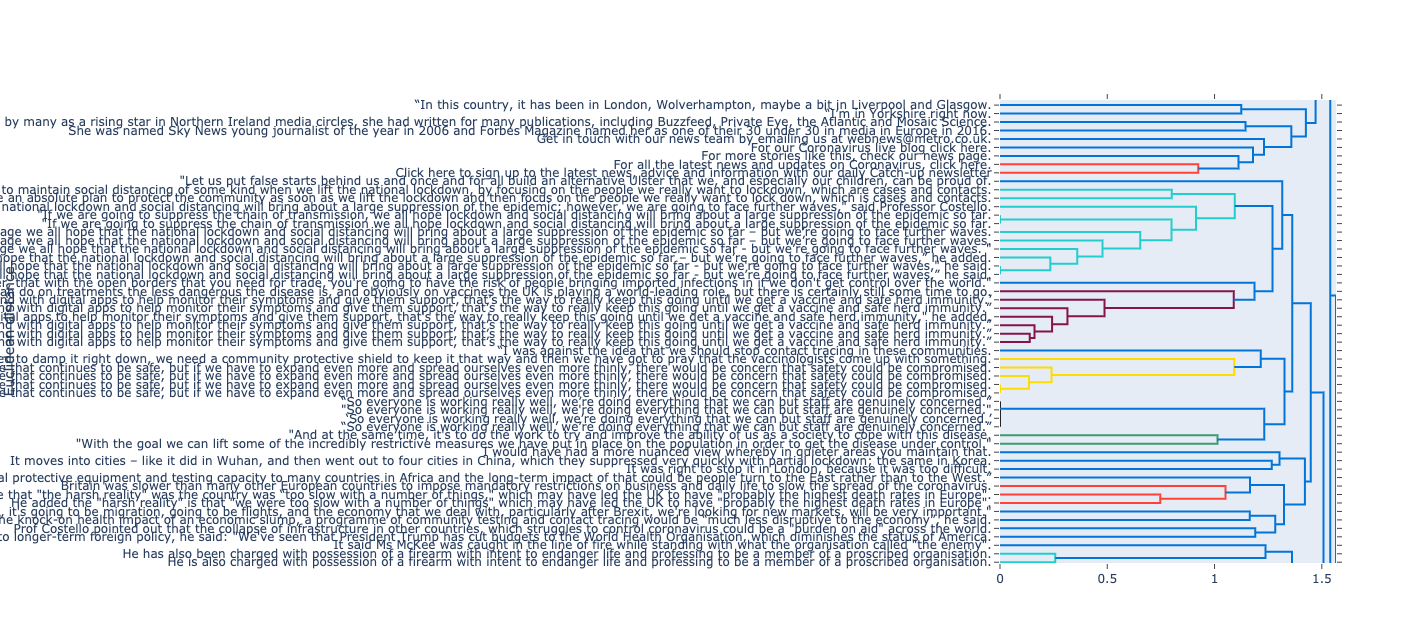
\includegraphics[width=\linewidth]{figures/dendrogram.png}
    \caption{A portion of the dendrogram that shows how different sentences are merged in the clusters by increasing distance values.}
    \label{fig:dendrogram}
\end{figure}

Using this type of inspection, we can decide specific threshold values more consistently: we can see what is the required similarity to make two pairs of sentences be in the same cluster.
% \todo{some observations about the distance values and threshold}

% 3. extract degree of uniqueness of words (from pairwise to clusterwise, with bag-of-words or difftool (order matters, duplicates))
% second motivation: highlight the different words and their uniqueness
With this method, we create sentence clusters that are very similar in their semantic content, but at the same time have linguistic changes.
To facilitate an analysis of the differences, we experimented with different methods of highlighting the uniqueness of the words in a cluster.
This can be seen in Figure~\ref{fig:words_uniqueness} where we score each of the words with a scale of uniqueness that is defined as:
$$u_w = 1 - \frac{|\Set{s_i | s_i \in S \land w \in s_i}|}{|S|}$$
where S is the set of sentences considered, $w$ is the word for which to compute the index. The expression compares the sentences of the current cluster where $w$ appears (numerator) with respect to the cluster size.
A value close to $1$ means that the word is used in just a few sentences in the cluster.
This gives a higher value of uniqueness to the word ``deceased'' that just appears in one over three sentences ($u = 2/3$), while ``surgery'' has $u = 0$.

\begin{figure}[!htb]
    \centering
    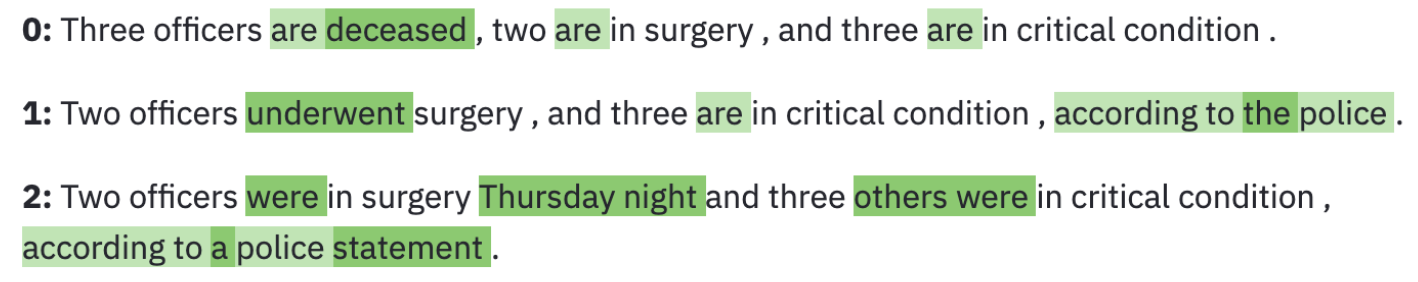
\includegraphics[width=\textwidth]{figures/words_uniqueness.png}
    \caption{A sentence cluster example, where the uniqueness of words in the cluster is highlighted with different shades of green.}
    \label{fig:words_uniqueness}
\end{figure}



% role of this experiment and outcomes
This methodology can be used in our framework to help the preparation of the dataset in different steps.
First of all, during the creation of article couples that have to be compared (using at the article-level the same clustering methodology). In this case, we will need to use a specific threshold that cuts out unrelated articles but at the same time keeps a considerable number of differences on the document level (not too similar because identical articles, that are a lot, are not useful).
While for the first user study we can exploit hand-curated groups of articles, when doing a larger creation of the dataset we will need to rely on automated techniques.
This methodology could also be used as support for the annotators, to see both which sentences are most similar, and the words that differ inside. This would make the annotation process faster and easier.

This experiment needs to be completed, to choose some parameters with better criteria. We want to identify good intervals for the thresholds and parameters (e.g. with euclidean distance around 0.6-1.0 sentences start to have linguistic variations but still very related to the same concepts).

This experiment evidences the need to explore more on the interpretation of the differences, pushing for the user study of RQ1.1.

It serves the RQ1.2 as a first implementation of the processing pipeline by making available different articles and their document and sentence-wise relationships. Building on top of these features, we can then develop the methodology for doing the cross-article framing analysis.




\subsection{Data collection}
% what
We also started collecting, early this year, several types of data that will be useful for the analysis planned.
% why
When looking for data, we are interested in different features.
First of all, a wide set of articles is needed, dense in time and from a wide variety of news outlets. We need substantial overlap between articles and the more sources we can include, the better we can observe variations of the framing phenomena.
Another very important feature is to have a good pre-clustered set of articles to help the curation of a dataset, especially for the first Research Question, by knowing that the articles are well related. Then when we will have the document clustering in action, this feature is not anymore required, but still can serve as a benchmark for that stage.
And another desirable feature would be to have articles that come from sources with a different opinion, that would be beneficial to create examples especially for the user study, where we want to maximise the occurrence of framing techniques. 

% how
% - google news (more than 500k articles) daily. Some stats about the number of sources involved  TODO: how is it made? What are its properties? Why useful?
Given these requirements and after exploring different news aggregators, we found that Google Headlines Full Coverage feature\footnote{\url{https://www.blog.google/products/news/new-google-news-ai-meets-human-intelligence/}} would fit the requirements of covering a big number of news sources (the \texttt{en-GB} version contains articles from more than 10k domains) and being very dense (an average of 9k new articles each day).
The data comes divided by topics (Latest, United Kingdom, World, Business, Technology, Entertainment, Sports, Science, Health) and inside each topic the articles are grouped in ``stories''. Each story has articles from the most relevant sources (``Top coverage'') and then lists also articles from other less important sources, for an average of 21 articles inside each story.
The stories are created automatically by Google News and this allows it to be always updated and be so diverse in the sources included.
We have captured from mid-march every day the published set of stories, and managed to retrieve more than 700k articles (as of the end of June, and not all the articles listed can be retrieved because of paywalls or other filtering techniques by the publishers).

% - allsides: human-created with interesting framing differences
Another data source that we actively retrieve is AllSides which provides a curated set of ``headlines''\footnote{\url{https://www.allsides.com/story/admin}} where three articles with a different political alignment are put together and compared in their difference.
The curators describe how the story gets framed by the considered sources, using natural language.
This description usually contains the usage of terms or themes that get mentioned.
At the end of June, we have available 4764 headlines, with 13979 articles linked.
Differently from Google Headlines which has different versions for each country, this data is US-focused being curated in the US and therefore has a much more limited scope. Also, the discussion of bias and framing is mainly focused on political issues, while we want to focus also on other types of differences of opinion.
% role of this specific data
This data, although the description of the differences is not directly parseable, will be used to feed the user study and understand the role of comparing different sides.

% - allnews: standard benchmark, wide adopted (find refs)

% scraping is legal for research: https://aballatore.space/2020/04/01/web-scraping-is-legal/

% role of this
The data collection done in these current months will continue across the PhD, and will be used in different stages of the analysis. It will serve as the seed to create the labelled dataset for the first Research Question and also provide a wide set of articles from different news sources to empower the studies of the second Research Question.
Having articles from so many different news sources, we can on one side provide some indication of framing for news sources that are not usually targeted by manual framing studies because not enough ``important'', and on the other side be more confident to observe some phenomenon of information re-usage that is the underlying hypothesis for the last sub-question.

\subsection{Formalisation and dissemination}
% what
The last type of activity carried out during this year has been the presentation of this work to other researchers throughout different events, both internally to the Open University and externally.
% why
The motivation of this activity has been to get some feedback from both people working inside the same research space and also from other fields.
From the first group, we wanted to get an expert opinion and mainly understand if we are missing some related research work that could be helpful.
Instead, from the more general-audience group, we wanted to understand if this type of research makes sense to them and try to explain more motivationally and in an easier format.

% how
Belonging to the first group, this work has been presented firstly to an internal seminar in KMi on the 25th March, then to the Text2Story workshop part of the ECIR conference as a position paper which was presented in April\footnote{\url{http://text2story20.inesctec.pt/}}.
This position paper~\cite{mensio2020towards} focuses on describing some proposed cross-article signals that would show differences in how stories are narrated.
The proposal described completely in this report has also been presented in the CRC PhD Conference, that is an internal conference for PhD students of KMi and C\&C schools.

For the more wide audience instead, during June we submitted a poster to the OU PhD Poster Competition which, involving a more general audience, focused more on being simple to understand.

These documents can be found at the end of this file.






\section{Plan}

% realistic
% clearly stated milestones
% dependencies explicit
% contingency planning – risks identified
% timeline – dates
% resources
% skills
% pretty presentation

In Figure~\ref{fig:gantt} we show the time plan, which mirrors the structure of the research questions.

The first phase will target RQ1.1, by doing the user study proposed before. This will require different stages, from the preparation of the data to be annotated and guidelines for the participants, to a small pilot to correct potential errors in the procedure, to the real user study and analysis of the results.

The outputs of the first phase will be needed by the second one, to create and annotate a larger dataset with the specific labels refined with the first study. The implementation of the pipeline is independent of this requirement so it can be done in parallel. The implementation of the detection model will sit on top of the pipeline.

After a month of buffer time, the analysis of the second research question will be faced, with two cycles of data preparation, implementation and analysis.

We plan for each of the groups to use the results of the analysis in papers that will be submitted to upcoming conferences.

The last six months will be dedicated exclusively to writing the thesis.

% \begin{landscape}
\begin{figure}[!htb]
    \centering{
    \resizebox{0.92\textwidth}{!}{
        \begin{ganttchart}[
            % y unit title=1cm,
            % y unit chart=1cm,
            vgrid,
            hgrid,
            time slot format=isodate-yearmonth,
            time slot unit=month,
            % title/.append style={draw=none, fill=barblue},
            % title label font=\sffamily\bfseries\color{white},
            % title label node/.append style={below=-1.6ex},
            % title left shift=.05,
            % title right shift=-.05,
            % title height=1,
            bar/.append style={draw=gray!50, fill=blue!50},
            % bar incomplete/.append style={fill=green}
            % bar height=.6,
            bar label font=\normalsize\color{black!50},
            % group right shift=0,
            % group top shift=.6,
            % group height=.3,
            % group peaks height=.2,
            group/.append style={draw=black, fill=black!50},
            vrule label font=\small,         % <---
            title label font=\small,         % <---
            bar label font=\small, 
            % inline,
  inline bar label node/.append style={
    align=center,
    right=30pt
  },
       ]{2020-07}{2022-09}
       \gantttitlecalendar{year, month}\\
        %   \ganttbar[
        %     progress=100,
        %     bar progress label font=\small\color{barblue},
        %     bar progress label node/.append style={right=4pt},
        %     bar label font=\normalsize\color{barblue},
        %     name=pp
        %   ]{Preliminary Project}{2020-09}{2020-12} \\
        % \ganttset{progress label text={}, link/.style={black, -to}}
        % \ganttgroup{Pipeline}{2020-07}{2020-12} \\
        %     \ganttbar[name=T0]{Implementation}{2020-07}{2020-12} \\
            % \ganttlinkedbar[progress=0]{Task B}{2021-07}{2021-12} \\
        \ganttgroup{RQ1.1}{2020-07}{2020-11} \\
            \ganttbar[]{User study preparation}{2020-07}{2020-09} \\
            \ganttlinkedbar[]{Pilot}{2020-9}{2020-9} \\
            \ganttlinkedbar[]{User Study}{2020-10}{2020-10} \\
            % \ganttbar[progress=0]{RQ1.2: Hypothesis}{2020-07}{2020-12} \\
            \ganttlinkedbar[name=res11]{Results analysis + paper}{2020-10}{2020-11} \\
            % \ganttlink[link mid=.4]{T0}{T12}\\
            % \ganttbar[]{RQ1.2: Analysis}{2021-02}{2021-03} \\
        \ganttgroup{RQ1.2}{2020-07}{2021-05} \\
          \ganttbar[]{Pipeline}{2020-07}{2020-09}\\
            \ganttlinkedbar[name=model12]{Dataset building}{2020-12}{2021-02}\\
            \ganttbar[name=model12]{Model implementation}{2020-12}{2021-02}\\
            % \ganttbar[progress=0]{RQ1.2: Hypothesis}{2020-07}{2020-12} \\
            \ganttlinkedbar[name=output12]{Analysis + paper}{2021-03}{2021-05}\\
            %\ganttlinkedbar[]{Online tool}{2021-03}{2021-04} \\
        
          
        \ganttgroup{RQ2.1}{2021-07}{2021-10} \\
          \ganttbar[name=model21]{Data retrieval and implementation}{2021-07}{2021-08}\\
          \ganttlinkedbar[]{Analysis + paper}{2021-09}{2021-10}\\
          
        \ganttgroup{RQ2.2}{2021-11}{2022-02} \\
          \ganttbar[name=model22]{Implementation}{2021-11}{2021-12}\\
          \ganttlinkedbar[]{Analysis + paper}{2022-01}{2022-02}\\
          
        \ganttgroup{Thesis}{2022-04}{2022-09} \\
          \ganttbar[]{Writing}{2022-04}{2022-09}
          
         \ganttlink[]{res11}{model12}
         \ganttlink[]{output12}{model21}
         \ganttlink[]{output12}{model22}
    \end{ganttchart}}}
    \caption{Gantt chart showing the time plan}
    \label{fig:gantt}
\end{figure}
% \end{landscape}

